\documentclass[10pt,a4paper]{article}
\usepackage[margin=13mm,top=12mm,bottom=14mm]{geometry}
\usepackage{graphicx,xcolor,tabularx,booktabs,array,enumitem,microtype,lmodern,fancyhdr}
\usepackage[T1]{fontenc}
\setlength{\parindent}{0pt}\setlength{\parskip}{3pt}
\setlist{leftmargin=5mm,itemsep=1pt,topsep=2pt}
\definecolor{navy}{HTML}{17365D}\definecolor{blue}{HTML}{2F75B5}
\definecolor{green}{HTML}{548235}\definecolor{amber}{HTML}{BF8F00}
\definecolor{red}{HTML}{C00000}\definecolor{gray}{HTML}{666666}
\definecolor{pb}{HTML}{E7F0F8}\definecolor{pg}{HTML}{EAF2E3}
\definecolor{pa}{HTML}{FFF3D6}\definecolor{pr}{HTML}{FBE5E5}\definecolor{px}{HTML}{EEEEEE}
\newcommand{\boxx}[2]{\colorbox{#1}{\parbox{\dimexpr\linewidth-2\fboxsep}{#2}}}
\newcommand{\headx}[1]{{\color{navy}\LARGE\bfseries #1}\par\vspace{1mm}{\color{blue}\rule{\linewidth}{1.1pt}}\vspace{2mm}}
\newcommand{\status}[2]{\colorbox{#1}{\textcolor{white}{\bfseries\scriptsize #2}}}
\pagestyle{fancy}\fancyhf{}\lhead{\footnotesize Detailed supervisor progress report}
\rhead{\footnotesize 24 July 2026}\cfoot{\footnotesize\thepage\ / 12}
\renewcommand{\headrulewidth}{.3pt}
\begin{document}

\headx{Technical Progress Report}
{\Large\bfseries Adaptive Remeshing, MISESERI Refinement, and State Transfer\par for Phase-Field Fracture in Abaqus\par}
\begin{tabularx}{\linewidth}{@{}lX@{}}
\textbf{Author} & Pruthviraja Reddy Vandavagali\\
\textbf{Programme} & Master Thesis, TU Bergakademie Freiberg\\
\textbf{Purpose} & Detailed technical progress and current evidence boundary\\
\end{tabularx}
\begin{minipage}[t]{.56\linewidth}
\textbf{Model and objective.} A $1\times1$ mm single-edge-notched plate is opened in Mode I using a layered phase-field fracture implementation. The computational objective is to reduce cost by MISESERI-guided local refinement while preserving mesh topology, irreversible state, and a defensible force--displacement response.

\boxx{pg}{\textbf{\color{green}Validated scope.} Technical reproduction; elastic, pre-peak and peak Stage C response; controlled state ingestion; bounded pre-peak nonmatching transfer; offline active-set correction under frozen history.}
\boxx{pr}{\textbf{\color{red}Evidence boundary.} Post-peak crack-path equivalence, corrected mechanical restart, D3E, and online adaptive remeshing are not established.}
\end{minipage}\hfill
\begin{minipage}[t]{.41\linewidth}\centering
\includegraphics[width=.88\linewidth]{../../results/supervisor_progress_update_detailed/figures/model_geometry_bc.pdf}\\[-1mm]
\footnotesize Single-edge split-notch benchmark and Mode-I opening.
\end{minipage}
\small
\begin{tabularx}{\linewidth}{@{}Xr@{}}\toprule
\textbf{Work package} & \textbf{Status}\\\midrule
Published UEL/UMAT framework and environment & \status{green}{COMPLETED}\\
MISESERI offline pre-refinement & \status{green}{VALIDATED IN SCOPE}\\
Nonmatching pre-peak state transfer & \status{green}{BOUNDED PASS}\\
Fixed active set through loading & \status{red}{DISPROVEN}\\
Offline obstacle correction & \status{green}{KKT PASS}\\
Corrected mechanical restart / online continuation & \status{gray}{UNPROVEN / WITHHELD}\\
Thesis integration and supervisor review & \status{blue}{ONGOING}\\\bottomrule
\end{tabularx}
\vfill\footnotesize Frozen evidence revision: \texttt{c34a944da4d01ba6a694878104b0c10c3d87f24e}.

\clearpage
\headx{1. Research question and model problem}
\begin{minipage}[t]{.47\linewidth}
\textbf{Research question.} Can an error-indicator-driven, locally refined mesh reproduce the useful mechanical response of the uniform reference with lower cost, and can the irreversible fracture state be moved to a nonmatching mesh without losing control of phase, history, ordering, or solver ingestion?

Phase-field fracture replaces a sharp crack with a regularized scalar field $d$. Refinement is difficult because the process-zone width is tied to the length scale $l_c$, while the Abaqus implementation contains three coincident element layers. Changing a mesh therefore changes not only geometry and connectivity but also physical/visualization namespaces and the ordering expected by Fortran. Restarting additionally requires the nodal phase and integration-point history to obey irreversibility.

\boxx{pa}{\textbf{Mesh roles.} H0 is the development mesh; H1 is the production comparison; H2-PUB is the finer published-family check. H1 remains the report reference even where refined-v3 reduces cost.}
\end{minipage}\hfill
\begin{minipage}[t]{.50\linewidth}\centering
\includegraphics[width=.72\linewidth]{../../results/supervisor_progress_update_detailed/figures/model_geometry_bc.pdf}
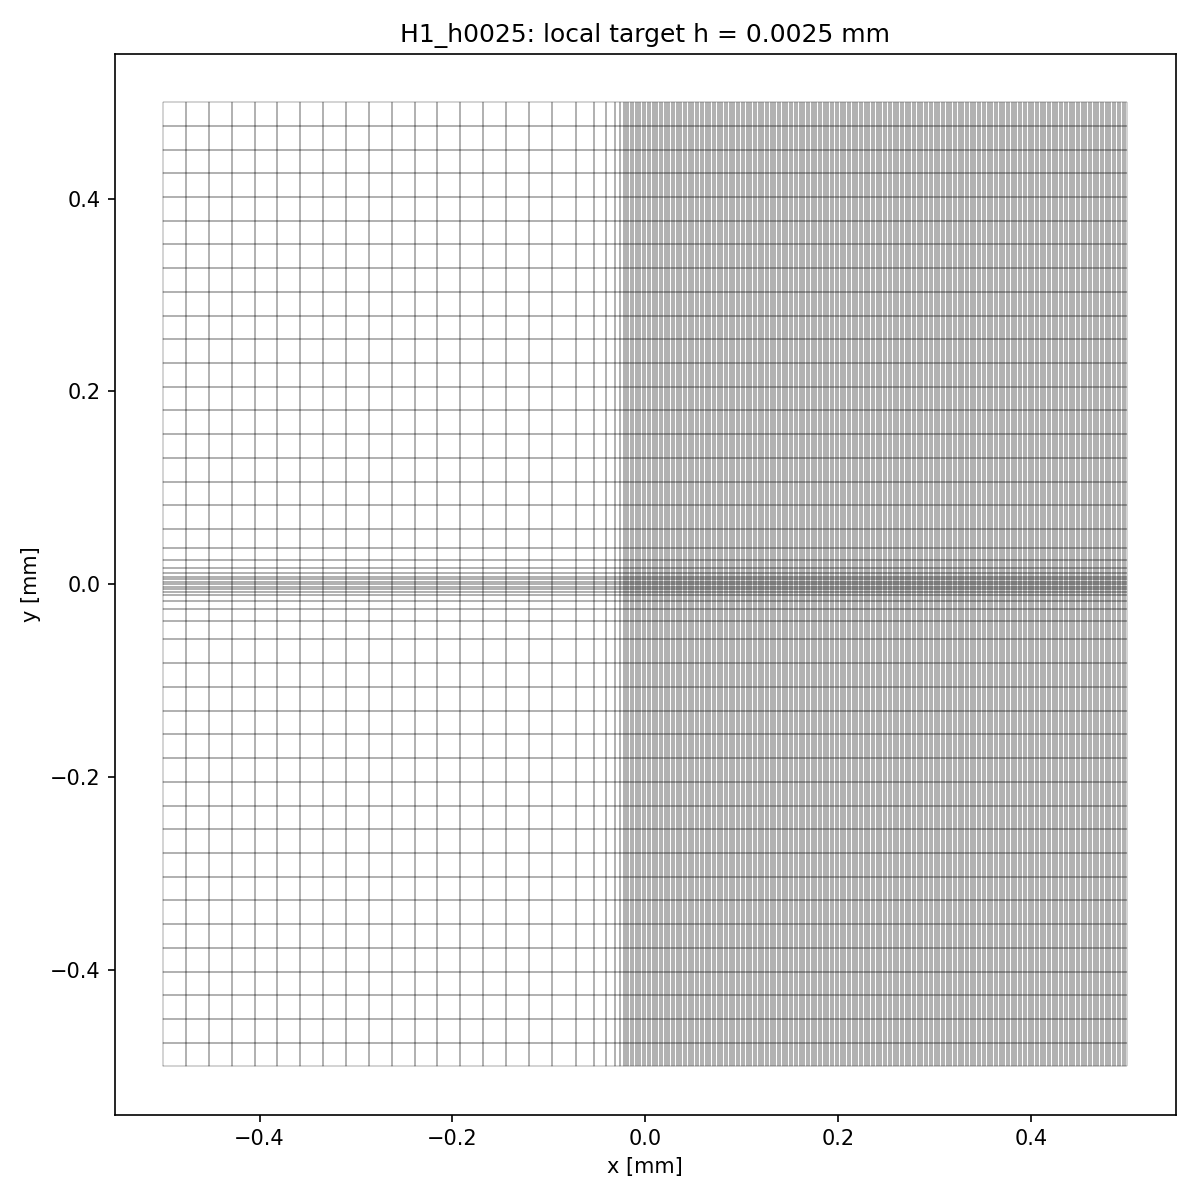
\includegraphics[width=.92\linewidth]{../../models/generated/molnar_gravouil_2017/h_convergence_lc015/H1_h0025/mesh_image.png}\\[-1mm]
\footnotesize H1 representative mesh; refinement is concentrated around the notch/process corridor.
\end{minipage}

\small
\begin{tabularx}{\linewidth}{@{}lXl@{}}\toprule
Quantity & Committed value & Meaning\\\midrule
Geometry & $1.0\times1.0$ mm, unit thickness & plane-strain plate\\
Notch & 0.5 mm split-node notch at $y=0$ & open free faces\\
Loading & $\alpha=90^\circ$ & pure Mode-I tension\\
$E,\nu$ & 210 kN/mm$^2$, 0.3 & linear elastic solid\\
$G_c,l_c$ & 0.0027 kN/mm, 0.0075 mm & fracture energy and regularization\\
H1 & 12,064 physical elements & production comparison\\
H0 / H2-PUB & 3,930 / 33,852 elements & development / finer check\\\bottomrule
\end{tabularx}
\boxx{pb}{\textbf{Control principle.} A result is accepted only when topology, complete field coverage, finite/bounded values, ordering, positive Jacobians, mechanical response, and the relevant KKT gates all support the same interpretation.}

\clearpage
\headx{2. Published framework and implementation architecture}
\begin{center}\includegraphics[width=.93\linewidth]{../../results/supervisor_progress_update_detailed/figures/uel_umat_information_architecture.pdf}\end{center}
\textbf{How information flows.} Python creates one physical mesh and reconstructs three coincident layers: U1 solves the phase field, U2 solves displacement/mechanics, and CPS4/UMAT exposes state variables for visualization and extraction. The Fortran element count and element/integration-point ordering must match the generated deck. Abaqus advances increments and supplies reaction-force and energy histories.

The mechanical layer uses displacement to obtain strain, stress, and the tensile history driver $H$. The phase layer uses $H$, the current phase $d$, and its gradient to solve the regularized fracture problem subject to irreversibility. SDV15 and SDV16 in the visualization layer carry the reported phase and history conventions. The runtime/UEXTERNALDB route loads prepared restart state where required; postprocessing independently audits coverage, ordering, RF--U, energy, phase bounds, and Jacobians.

\boxx{pb}{\textbf{Notation.} U1 and U2 here are coincident element-layer identifiers, not displacement components. Applied vertical displacement is written as $U_2$.}
\boxx{pa}{\textbf{Why the visualization layer matters.} User elements do not automatically provide ordinary contour fields. The coincident CPS4/UMAT layer makes $d$, $H$, stress, and related solution-dependent variables inspectable without changing the scientific UEL formulation.}
\boxx{pg}{\textbf{What was demonstrated.} The reconstructed layered implementation is technically reproducible, and later transfer tests show that prepared phase/history values reach the expected Abaqus output channels. This is implementation evidence, not a claim that arbitrary online remeshing is validated.}

\clearpage
\headx{3. MISESERI pre-refinement and mesh reconstruction}
\begin{center}
\includegraphics[width=\linewidth]{../../results/supervisor_progress_update_detailed/figures/miseseri_refinement_flow.pdf}\\
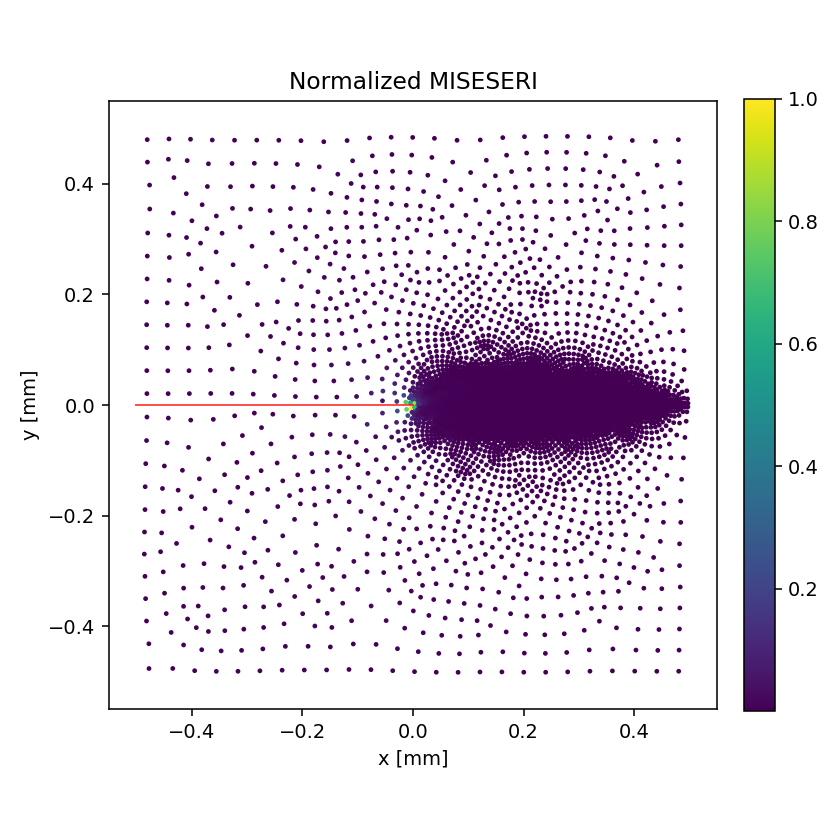
\includegraphics[width=.42\linewidth]{../../runs/hpc/stage_c_miseseri/molnar_h0_miseseri_preanalysis/evidence/1376296.mmaster02/figures/02_normalized_miseseri_contour.png}\hfill
\includegraphics[width=.42\linewidth]{../../results/supervisor_progress_update_detailed/figures/miseseri_threshold_elements.pdf}\\
\includegraphics[width=.57\linewidth]{../../results/supervisor_progress_update_detailed/figures/h1_refined_v3_near_notch_sampling.pdf}
\end{center}
An auxiliary continuum analysis produces MISESERI at physical elements. The committed rule normalizes by the maximum and marks the connected notch-tip component where $\mathrm{MISESERI}/\max(\mathrm{MISESERI})>0.05$. A graded mesh then uses $h_{\min}=0.0025$ mm and $h_{\max}=0.025$ mm in one refinement pass with no coarsening. U1, U2, and CPS4 layers are rebuilt, \texttt{N\_ELEM} is updated, and static guards check layer counts, sets, ordering, notch topology, and element orientation before solving.

\boxx{pr}{\textbf{Engineering lesson from C2F-v2.} Omitting the exact $y=0$ line removed the split-notch free faces. The resulting continuous plate was about 72\% too stiff and suppressed softening. Restoring the line and split topology corrected the geometry before C2F-v3. Mesh generation therefore treats topology as a scientific input, not merely a meshing detail.}
\boxx{pg}{\textbf{Output.} Refined-v3 contains 10,290 physical elements versus 12,064 for H1. The near-notch panels use committed element-centroid sampling from matched-state extractions to show the different local discretization patterns; they are not screenshots or reconstructed connectivity.}

\clearpage
\headx{4. Stage C mechanical response}
\begin{center}
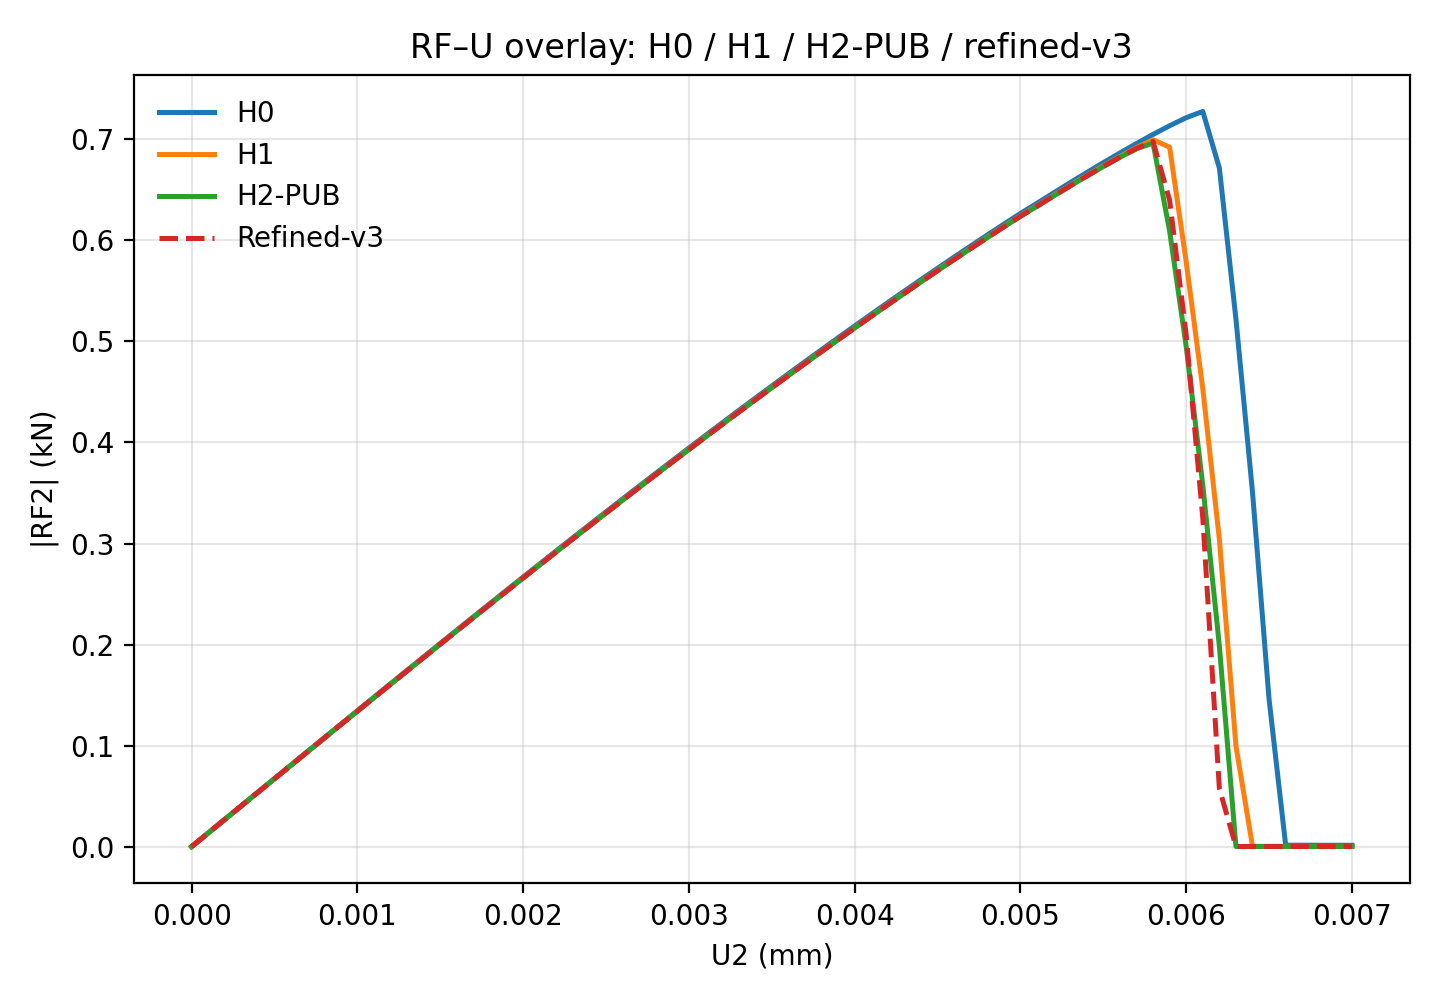
\includegraphics[width=.49\linewidth]{../../results/figures/stage_c_final/01_rf_u_h0_h1_h2_refined_v3.png}\hfill
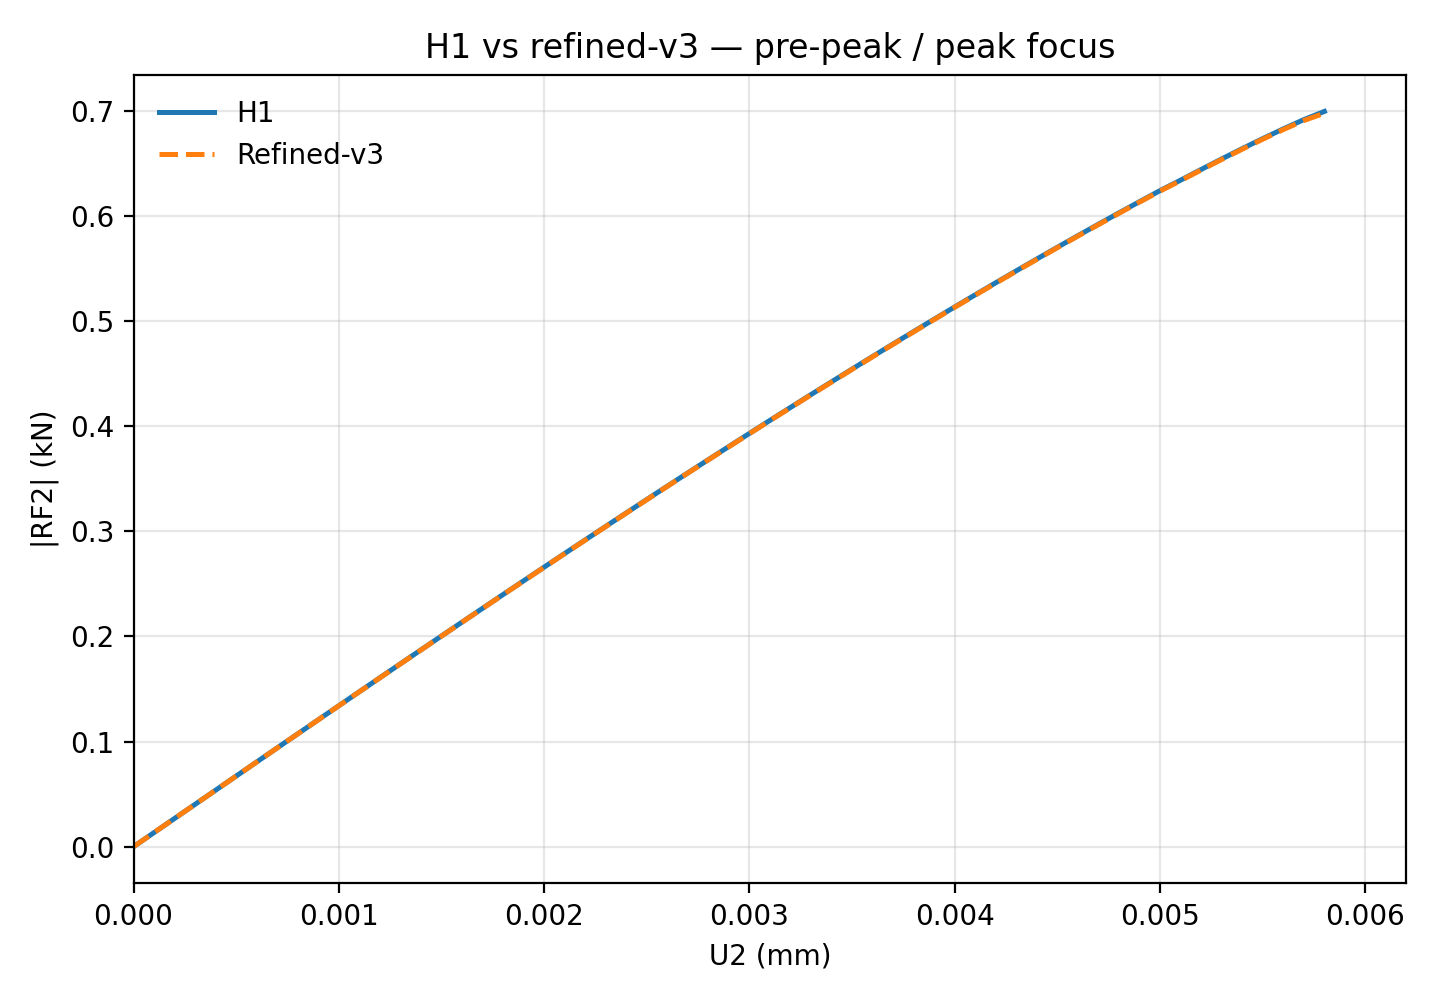
\includegraphics[width=.49\linewidth]{../../results/figures/stage_c_final/02_rf_u_h1_vs_refined_v3_prepeak.png}\\
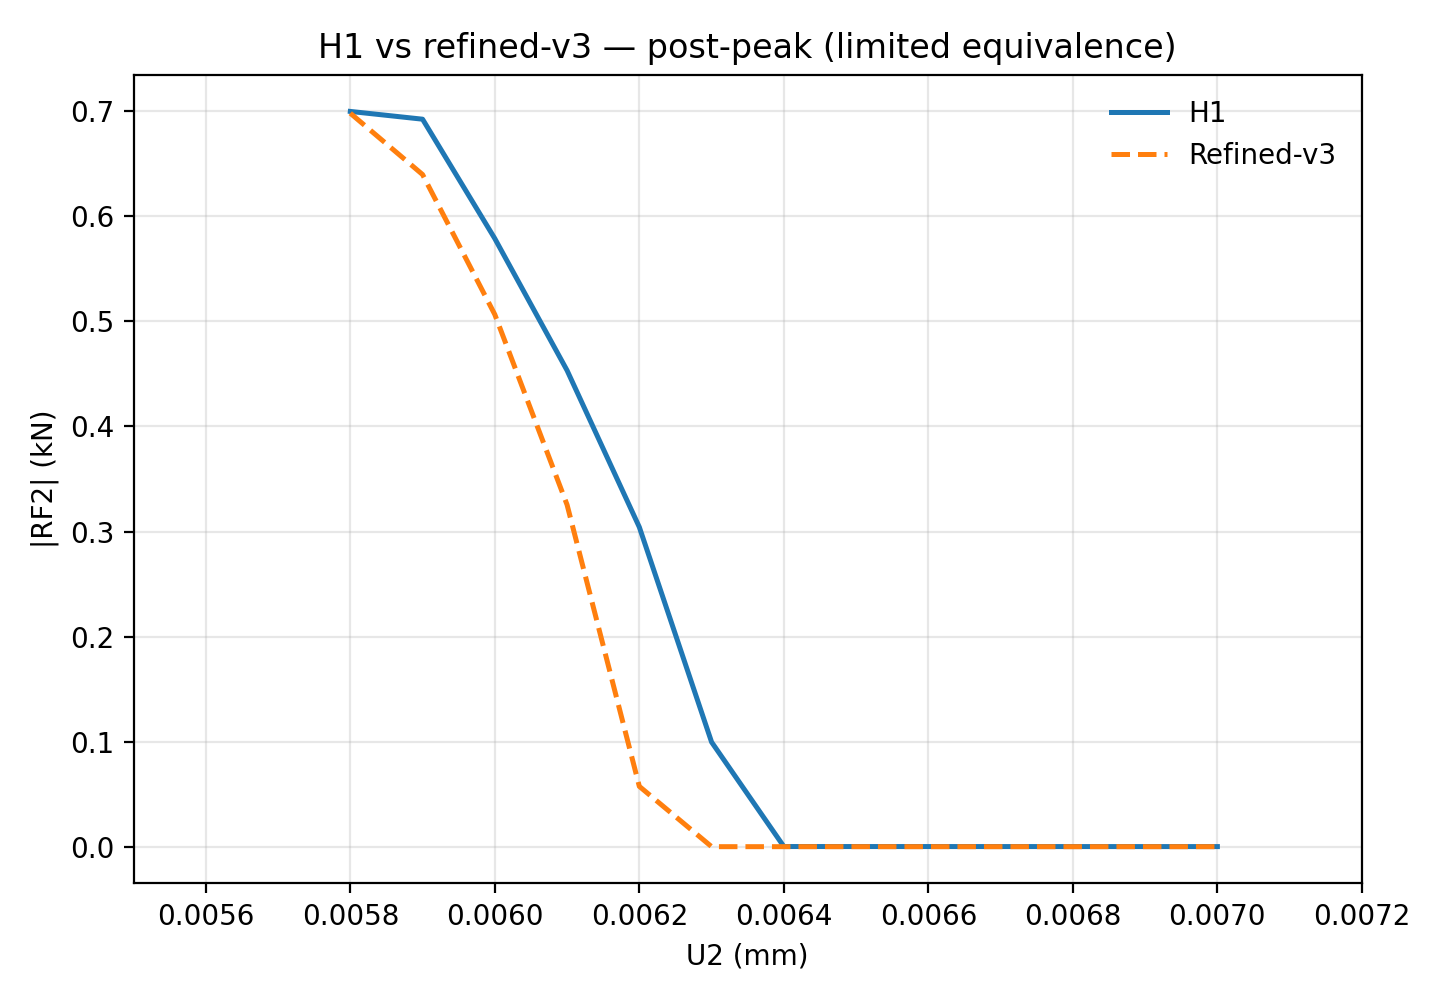
\includegraphics[width=.62\linewidth]{../../results/figures/stage_c_final/03_rf_u_h1_vs_refined_v3_postpeak.png}
\end{center}
\textbf{What was compared.} Refined-v3 and H1 were solved with the same four-thread execution basis and compared through reaction force versus imposed displacement (RF--U). The initial stiffness difference is 0.061\%, pre-peak normalized RMSE is 0.089\%, peak-force difference is 0.24\%, and both peak at $U_2=0.0058$ mm. These measurements support equivalence of the elastic branch, pre-peak evolution, and peak response within this parameter set.

After peak, localization becomes mesh- and path-sensitive. The post-peak NRMSE is approximately 24.3\%; the visibly different softening path prevents a post-peak-equivalence claim. The gate is intentionally separated: close pre-peak RF--U agreement does not imply identical crack evolution.

\boxx{pg}{\textbf{Supported.} Refined-v3 is validated for elastic, pre-peak, and peak RF--U response within the tested scope.}
\boxx{pr}{\textbf{Not supported.} It is not a crack-path-equivalent replacement for H1 and does not establish online remeshing.}

\clearpage
\headx{5. Stage C spatial and computational evidence}
\begin{center}
\includegraphics[width=\linewidth]{../../results/supervisor_progress_update_detailed/figures/stage_c_field_evidence.pdf}\\
\includegraphics[width=.55\linewidth]{../../results/supervisor_progress_update/figures/stage_c_efficiency_reductions.pdf}
\end{center}
The left field shows where the auxiliary indicator concentrates the proposed refinement. The matched $U_2=0.007$ mm contours show that both solutions propagate from the notch along the ligament, but their localized paths are not identical. At the SDV15 $\geq0.5$ threshold, H1 reaches 0.5075 mm and refined-v3 reaches 0.4949 mm; the Hausdorff distance is approximately 0.0122 mm. These are measured spatial differences, not plotting artifacts.

Against four-thread H1, refined-v3 uses 14.7\% fewer physical elements, 16.7\% less wall time, 14.9\% less CPU time, and 22.2\% less peak memory. These demonstrate measured efficiency for the frozen comparison, while queue/node/output effects mean they are not attributed universally to remeshing alone.

\boxx{pa}{\textbf{Interpretation.} Pre-peak global response is governed sufficiently well by the retained fine corridor. Post-peak localization amplifies small discretization/path differences, so force agreement at peak cannot be extrapolated to crack-path equivalence. H1 therefore remains the production reference.}

\clearpage
\headx{6. State-transfer formulation and information flow}
\begin{center}
\includegraphics[width=.94\linewidth]{../../results/supervisor_progress_update_detailed/figures/state_transfer_information_flow.pdf}\\[-1mm]
\includegraphics[width=.70\linewidth]{../../results/supervisor_progress_update_detailed/figures/checkpoint_phase_history_fields.pdf}
\end{center}
At the selected pre-peak source checkpoint, displacement/mechanical state, nodal phase $d$, and integration-point history $H$ are extracted with their mesh identities. Deterministic source-to-target mapping then interpolates or projects the nodal phase and maps history at integration points. Complete coverage and ordering audits prevent silent omission or layer mismatch; bounds and positive-Jacobian checks protect admissibility and geometry.

The target is a nonmatching split-notch package with 6,601 nodes, 6,400 physical elements, and 25,600 integration points. The \emph{recovered phase} is the transferred source field. It provides the irreversibility \emph{lower bound}; a \emph{compatible phase} may be corrected above that bound for the target discretization. History remains the actual transferred driving field. Active nodes are held at the lower bound; free nodes may change under the phase equilibrium equation.

\boxx{pa}{\textbf{Controlled analytical baseline.} Phase $L_2$/maximum errors are 0.027037/0.084997; history errors are 0.010797/0.023398. They are retained as measured baselines and are not described as negligible.}

\clearpage
\headx{7. Abaqus ingestion and bounded release hold}
\begin{minipage}[t]{.53\linewidth}
\textbf{Evidence sequence.} D2A proves that prepared phase and history are ingested through the Abaqus visualization state. D2B continues the tiny controlled model serially after one documented increment-limit correction. D2C repeats the accepted continuation with one MPI rank and four threads. D3 then transfers a real pre-peak fracture checkpoint to the nonmatching target; D3A3-R4 equilibrates it and performs a bounded compatible release hold.

The operation is checked at multiple levels: every target node and integration point is covered, field values are finite and bounded, element/IP ordering agrees, the split notch is retained, and no non-positive Jacobian occurs. SDV15 and SDV16 are compared against the prepared phase/history records. RF and energy jumps across release measure mechanical continuity over the bounded hold.

\boxx{pg}{\textbf{Result.} Maximum SDV15 transfer error is $1.3878\times10^{-17}$; SDV16 error is zero. Relative RF and energy release jumps are $2.2926\times10^{-4}$ and $1.2746\times10^{-5}$. Coverage is complete and no non-positive Jacobian is present.}
\end{minipage}\hfill
\begin{minipage}[t]{.44\linewidth}
\includegraphics[width=\linewidth]{../../results/supervisor_progress_update_detailed/figures/release_hold_rf_energy_continuity.pdf}
\small
\begin{tabularx}{\linewidth}{@{}Xr@{}}\toprule Gate & Outcome\\\midrule
Node/IP coverage & complete\\
Unmapped records & zero\\
Ordering audit & passed\\
Phase/history ingestion & passed\\
Serial/4-thread repeat & passed\\
Release RF jump & $2.2926\,10^{-4}$\\
Release energy jump & $1.2746\,10^{-5}$\\
Jacobian & all positive\\\bottomrule
\end{tabularx}
\end{minipage}
\boxx{pa}{\textbf{Boundary.} This validates bounded pre-peak ingestion and release hold. It does not validate arbitrary checkpoint transfer, post-peak continuation, or online remeshing.}
\begin{center}
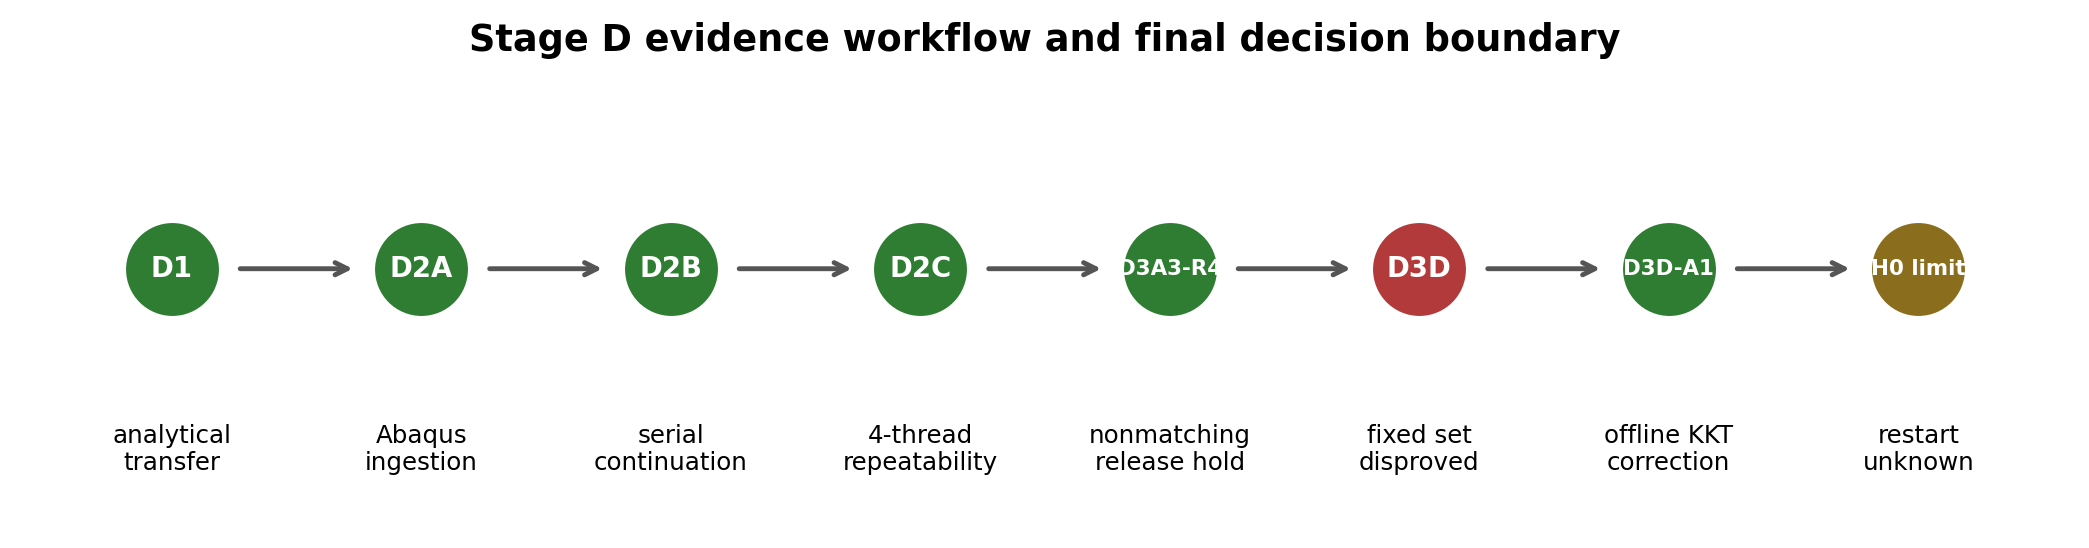
\includegraphics[width=.82\linewidth]{../../results/final/stage_d/figures/stage_d_workflow.png}\\[-1mm]
\footnotesize Evidence progression from controlled transfer to the bounded mechanical-restart limitation.
\end{center}

\clearpage
\headx{8. Active-set evolution: why a fixed set fails}
\begin{center}
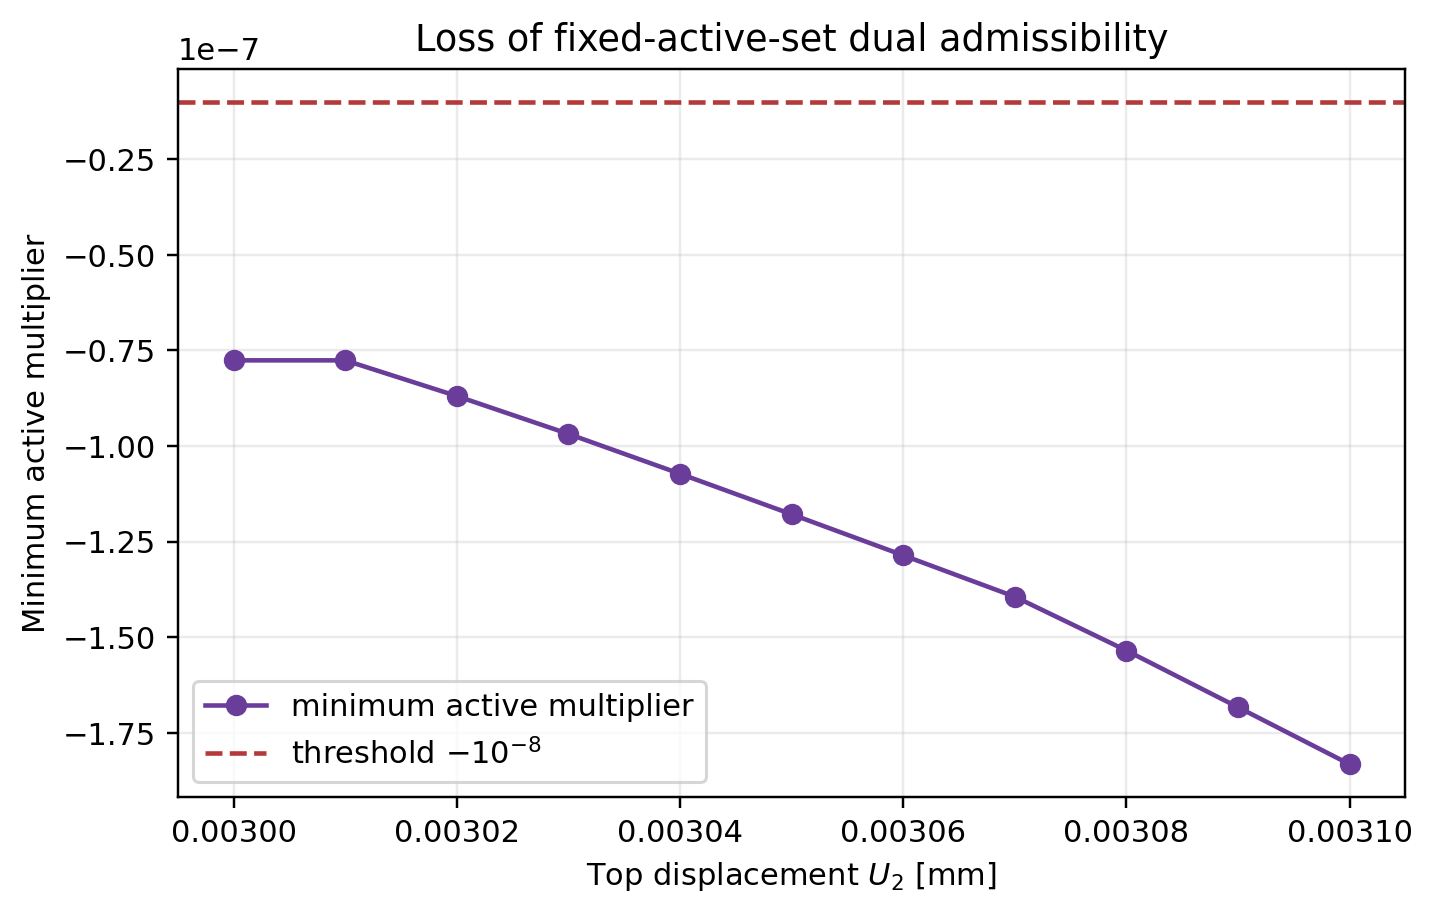
\includegraphics[width=.48\linewidth]{../../results/final/stage_d/figures/minimum_active_multiplier_vs_displacement.png}\hfill
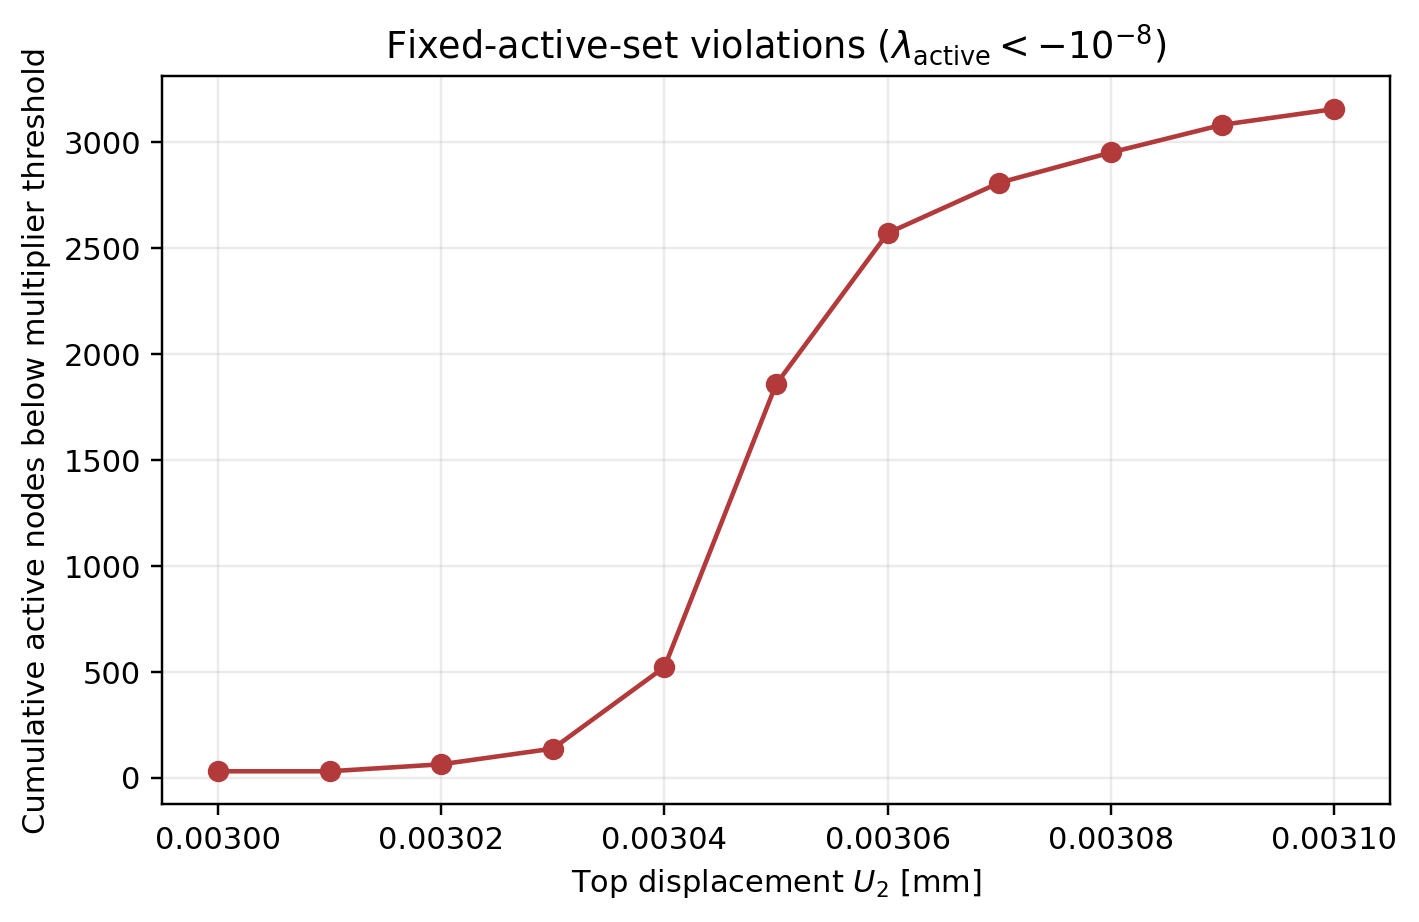
\includegraphics[width=.48\linewidth]{../../results/final/stage_d/figures/violating_active_nodes_vs_displacement.png}\\
\includegraphics[width=.48\linewidth]{../../results/supervisor_progress_update_detailed/figures/offline_correction_released_locations.pdf}
\end{center}
An active phase node is held at its irreversibility lower bound: it cannot heal below the recovered phase. Its multiplier measures whether that constraint is mechanically consistent. Under the frozen acceptance rule, an active multiplier below $-10^{-8}$ indicates that keeping the node fixed violates the KKT sign condition; that node must be released into the free set.

The first continuation frame already contains 30 violating active nodes. As loading advances, the cumulative count grows to 3,157 and the minimum multiplier reaches $-1.8327\times10^{-7}$. The spatial pattern is not a numerical label change: it identifies where the target phase equilibrium wants to move away from the inherited bound.

\boxx{pa}{\textbf{Population distinction.} The 72 plotted locations are the converged release set from the subsequent offline correction, not the full population of 3,157 endpoint violations in the continuation test.}
\boxx{pr}{\textbf{Conclusion.} A fixed active set through the tested loading segment is disproven. Passing irreversibility, residual, lower-bound, and Jacobian checks is insufficient when the active-multiplier sign gate fails.}

\clearpage
\headx{9. Offline primal--dual active-set correction}
\begin{center}
\includegraphics[width=.60\linewidth]{../../results/supervisor_progress_update_detailed/figures/active_set_iteration_history.pdf}\hfill
\includegraphics[width=.36\linewidth]{../../results/supervisor_progress_update_detailed/figures/offline_correction_released_locations.pdf}
\end{center}
The correction begins with the recovered F3 phase as the unchanged irreversibility lower bound and the actual F3 history field. At each primal--dual iteration, nodes with inconsistent active multipliers are released, the free phase equations are solved, and residual, bound, phase-decrease, and Jacobian gates are reevaluated. This separates mathematical phase admissibility from subsequent mechanical restart acceptance.

The update converges deterministically in seven iterations to 6,374 active and 227 free nodes. All 30 original violating seeds and 42 additional nodes are released; no released node was reactivated during the iteration. Intermediate free residuals are recorded as infinite until membership stabilizes, so the figure reports membership changes rather than implying a finite residual history. At iteration 7, the evaluated free residual is $2.1176\times10^{-21}$, the minimum active multiplier is $-9.99696\times10^{-9}$ (inside the $-10^{-8}$ gate), and active-bound error is zero. There is no phase decrease or non-positive Jacobian, and the phase functional decreases.

\boxx{pg}{\Large\bfseries The corrected phase field is KKT-admissible under the frozen F3 history.}
\boxx{pr}{\Large\bfseries The candidate has not been mechanically re-equilibrated and is therefore not an accepted Abaqus restart.}
\small KKT denotes Karush--Kuhn--Tucker conditions. The offline result proves the obstacle update only; mechanical equilibrium could change displacement, history, and the subsequent active set.

\clearpage
\headx{10. Execution limitation, lessons, and claim boundary}
\small
\begin{tabularx}{\linewidth}{@{}p{18mm}XXX@{}}\toprule
Job & Immediate cause & Prevention rule & Scientific output\\\midrule
1378003 & Windows/LF-dependent checksum comparison & derive/compare hashes in one Linux checkout & Abaqus not launched; none\\
1378004 & assignment expression under Python 3.6 & bind a qualified interpreter before validation & Abaqus not launched; none\\
1378005 & Git unavailable after module purge/load & login-side checks; pre-stage files; no compute-node Git & Abaqus not launched; none\\\bottomrule
\end{tabularx}
\normalsize
\textbf{What was learned.} These failures occurred in the wrapper/environment gates, before solver execution. Qualification must therefore isolate the environment from the scientific package: resolve repository state on the login node, pre-stage immutable inputs, bind Python/compiler/Abaqus explicitly, and execute a trivial callback/datacheck before consuming permission for a scientific restart. The failures do not contradict the offline KKT result because they generated no Abaqus state. The remaining scientific question is whether the corrected phase can be mechanically re-equilibrated while preserving actual-history KKT consistency.

\begin{minipage}[t]{.48\linewidth}
\boxx{pg}{\textbf{\color{green}Validated within scope}\\
Published framework reproduction; Stage C elastic/pre-peak/peak RF--U; controlled ingestion; bounded nonmatching pre-peak transfer; R4 release hold; offline active-set correction under frozen history.}
\end{minipage}\hfill
\begin{minipage}[t]{.48\linewidth}
\boxx{pr}{\textbf{\color{red}Disproven or withheld}\\
Fixed active set is disproven. Corrected mechanical restart, D3E, post-peak equivalence, equivalent crack path, online adaptive remeshing, and ABAQUSER comparison remain unproven, not performed, or withheld.}
\end{minipage}
\boxx{pa}{\textbf{Decision boundary.} The numerical evidence remains frozen. No further datacheck is authorized by this report. Reopening requires a separate decision after an independent environment gate passes.}
\begin{center}
\includegraphics[width=.78\linewidth]{../../results/supervisor_progress_update/figures/qualification_failure_timeline.pdf}
\end{center}
\boxx{pb}{\textbf{Permanent qualification chain.}\quad
Login-side provenance and hashes $\rightarrow$ explicitly bound interpreter/compiler/Abaqus
$\rightarrow$ one-element callback datacheck $\rightarrow$ only then consider a separately authorized scientific checkpoint. Each gate has a hard stop and preserves its own evidence.}

\clearpage
\headx{11. Next work and four-to-six-week reporting plan}
\begin{minipage}[t]{.48\linewidth}
\boxx{pb}{\textbf{\color{blue}Track A -- independent environment qualification}
\begin{enumerate}
\item Build the smallest one-element UEL/UMAT example.
\item Pre-stage deck, Fortran, wrapper, hashes, and manifests on the login node.
\item Use no compute-node Git; bind absolute Python, compiler, and Abaqus paths.
\item Run only a trivial user-subroutine datacheck and verify callback/module loading.
\item Retain stdout/stderr, environment/module inventory, checksums, solver command, and status.
\item \textbf{Pass:} Abaqus datacheck reaches normal completion with the callback loaded. \textbf{Stop:} any pre-Abaqus or callback failure; no scientific retry.
\end{enumerate}}
\end{minipage}\hfill
\begin{minipage}[t]{.48\linewidth}
\boxx{pg}{\textbf{\color{green}Track B -- thesis development}
\begin{enumerate}
\item Obtain comments on the consolidated tolerance policy.
\item Integrate validated Stage C/D evidence into the university template.
\item Complete theory/literature links for refinement, transfer, and active-set control.
\item Finalize discussion, limitations, conclusions, outlook, nomenclature, and references.
\item Prepare the defense presentation from the frozen claim matrix.
\end{enumerate}}
\end{minipage}

\vspace{3mm}
\begin{tabularx}{\linewidth}{@{}p{22mm}X@{}}\toprule
Window & Milestone\\\midrule
Week 1 & Package and review the one-element qualification gate; integrate supervisor comments.\\
Week 2 & If separately authorized, execute only the gate and preserve evidence; otherwise continue writing.\\
Weeks 3--4 & Complete methodology/results integration, literature context, and claim-matrix cross-check.\\
Weeks 5--6 & Resolve layout/references, produce supervisor draft, and prepare defense visuals.\\\bottomrule
\end{tabularx}

\boxx{pa}{\Large\bfseries The work has established a reproducible, bounded workflow for offline MISESERI refinement and pre-peak state transfer. The remaining technical question is the mechanically qualified restart after active-set correction; post-peak and online-remeshing claims remain withheld.}
\vfill\footnotesize This report is a detailed progress update, not the final thesis. It authorizes no HPC or Abaqus execution.

\end{document}
